\startchapter{Introduction to the LHC and the ATLAS Detector}
\label{chapter:lhc_atlas}

The Large Hadron Collider (LHC) \cite{lhc_machine} is a circular proton-proton collider which resides in a 27 km tunnel near the European Organization for Nuclear Research (CERN). Superconducting magnets are used to accelerate counter-rotating bunched proton beams to near the speed of light, and direct the beams into head-on collisions at four interaction points around the ring. The collisions take place at a world-leading centre of mass energy of up to 13 TeV. Each interaction point is surrounded by a detector, which measures the energetic debris of particles produced by the high energy collisions to perform precision measurements of the SM and search for new physics.

The large 13 TeV centre of mass energy of the collisions makes it possible for the colliding proton constituents, known as ``partons", to pair annihilate and subsequently produce massive unstable particles such as the Higgs boson, which cannot presently be produced by any other experimental means. By studying potential decay products of hypothesized massive particles that could be produced at the LHC, experiments at the LHC can study hypothesized DM production mechanisms which would proceed via the decay of these massive particles. 

The LHC also collides protons at a world-leading collision rate - also known as instantaneous luminosity, see Section zzz - of $10^{34}$cm$^{-2}$s$^{-1}$, $\sim$100 times higher than the next-leading proton-proton collision rate at the Tevatron collider \cite{tevatron} which operated from 1983-2011. Over several years of data-taking the high collision rate at the LHC has enabled experiments to collect statistics-rich data sets. These large data sets enable searches for new physics to study highly selective subsets of the data in which signatures of new physics are predicted, while still maintaining a sufficient amount of data in these subsets to make statistically significant comparisons with Standard Model predictions to search for excesses in the data that could point to new physics.

\section{Parton Model}

The proton has an internal structure comprised of constituent quarks, antiquarks and gluons - collectively known as ``partons" - and their interactions \cite{parton_model}. When a proton collides with another particle in particle colliders such as the LHC, the probability density $f(x, Q^2)$ that a particular species of parton, for example a quark with ``up" flavour $u$, will be involved in the collision is a function of both the fraction $x$ of the proton's momentum carried by the parton, and the squared momentum scale $Q^2$ of the collision. Detailed parameterized models of the parton distribution function (PDF), such as MSHT20 \cite{MSHT20} have been developed using combined fits to data from deep inelastic scattering (DIS) experiments at proton colliders. MSHT20 PDF models at $Q^2$ of 10 GeV$^2$ and $10^4$ GeV$^2$ are shown in Figure \ref{fig:msht20_pdfs}.

\begin{figure}[H]
	\centering
	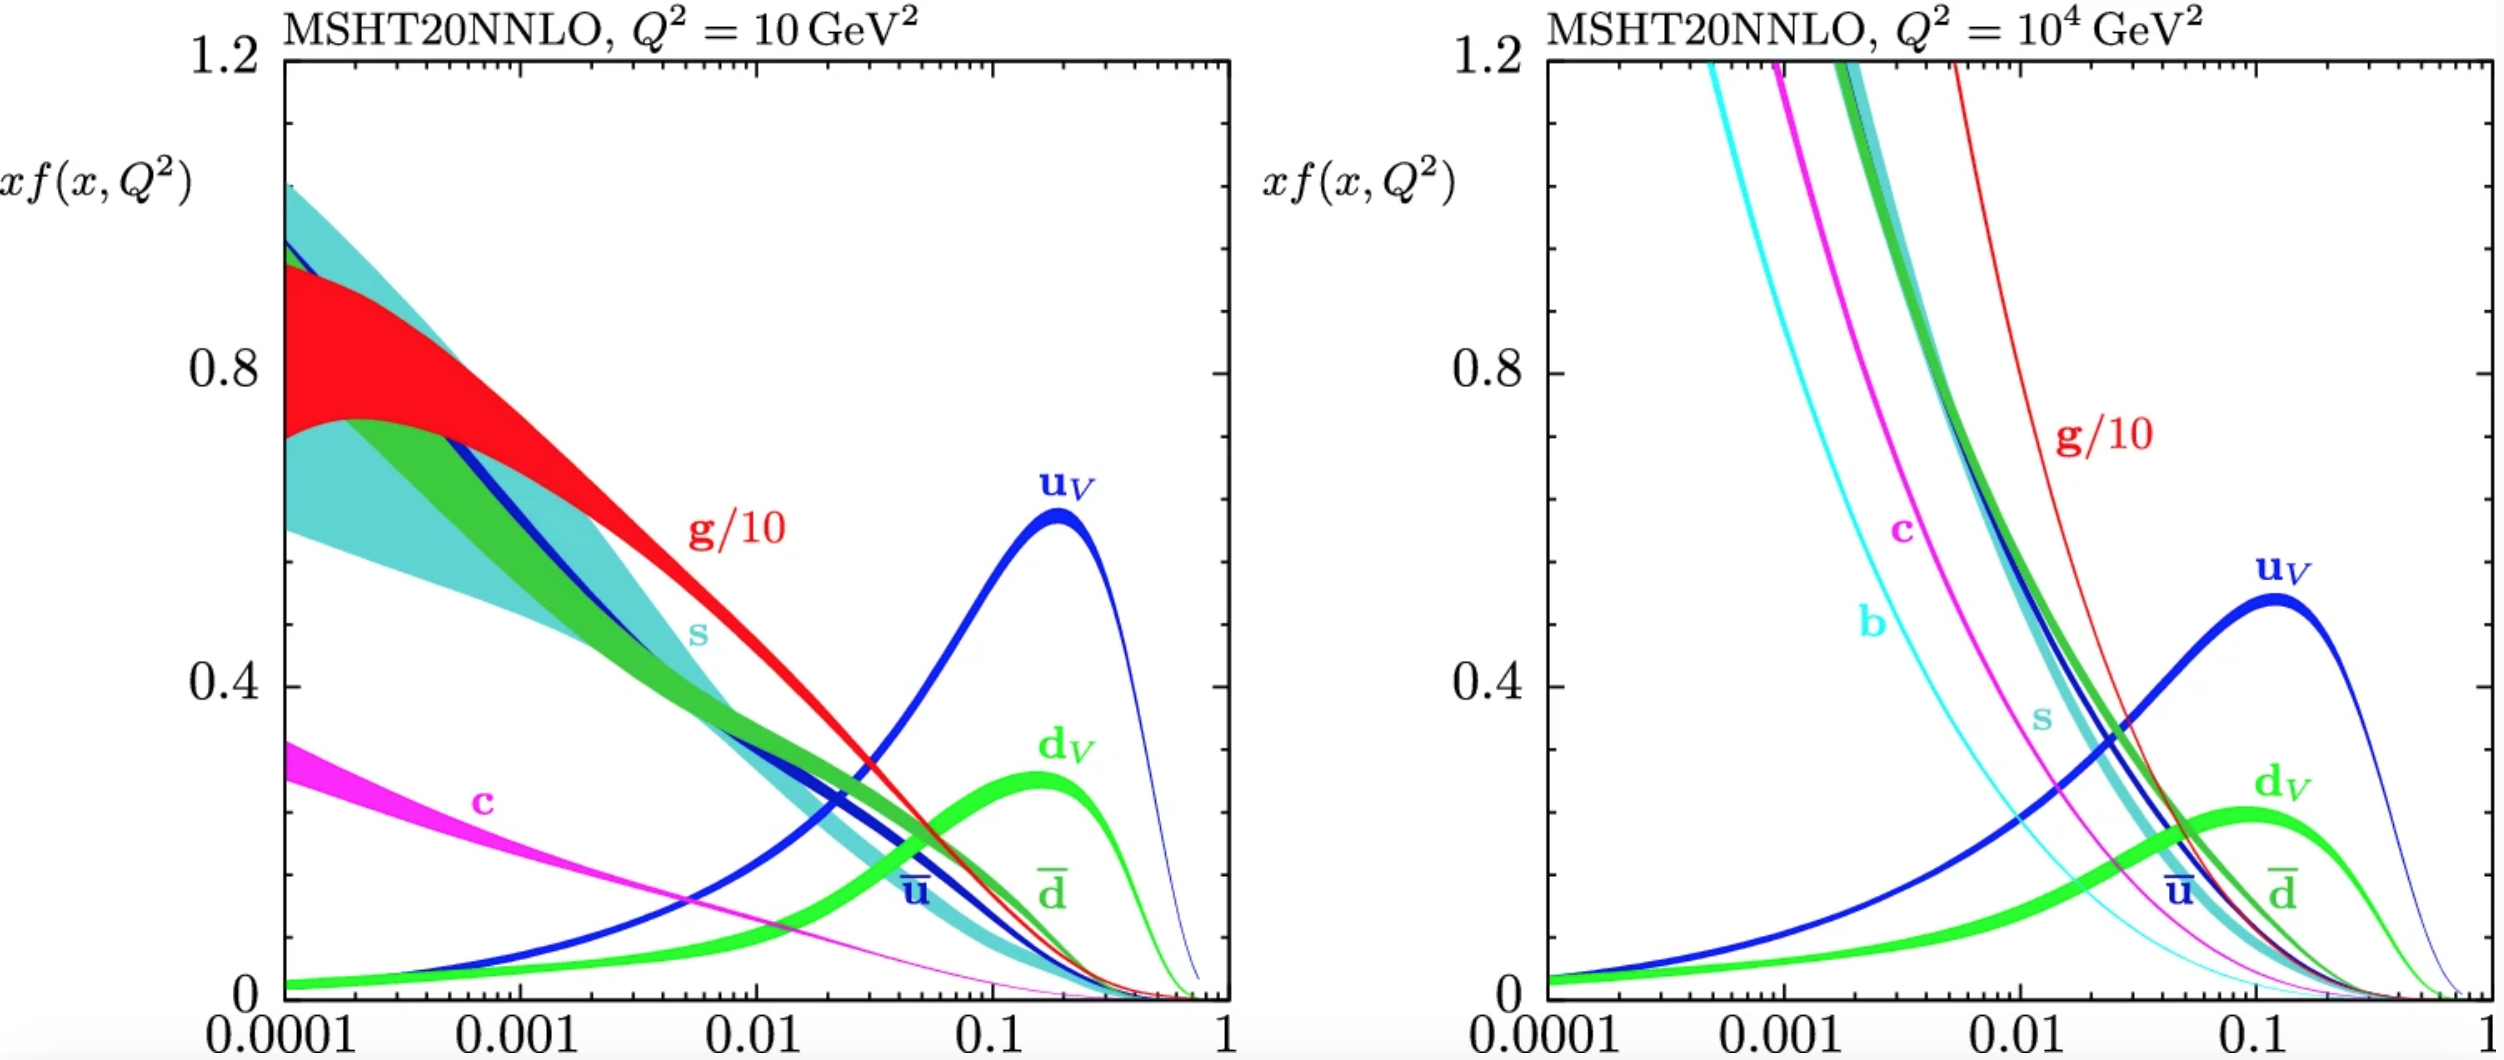
\includegraphics[width=0.9\textwidth]{Figures/3/MSHT20_PDFs.png}
	\caption[]{Parton distribution functions modelled with MSHT20 at $Q^2=10$ GeV$^2$ and $10^4$ GeV$^2$}.
	\label{fig:msht20_pdfs}
\end{figure}

Based on the PDFs shown in Figure \ref{fig:msht20_pdfs}, $u$ and $d$ quarks carry the highest probability density for parton momentum fractions above $\sim$10\%, with the $u$ carrying approximately double the probability density of the $d$. These dominant quarks are known as the proton's ``valence" quarks, of which there are two $u$ and one $d$, and they carry the proton's quantum numbers.

\section{Decay Processes from Parton Collisions}

Each process of particle production initiated by high-energy particle collisions at the LHC proceeds with a certain probability relative to other processes that could also be initiated by the same collision. The probability that a given process will take place is quantified by its ``cross section" $\sigma$. The beam luminosity $\mathcal{L}$ relates the rate of collisions $\frac{dN}{dt}$ which proceed via a given process to the cross section of the process:

\begin{equation}
\frac{dN}{dt} = \mathcal{L}\sigma
\end{equation}

The luminosity can be integrated over a period of time $t_1$ to $t_2$, such that the total number of events expected to be produced via a process with cross section $\sigma$ over the given period is related to the ``integrated luminosity" $\mathcal{L}_\text{int}$ by:

\begin{equation}
N = \sigma\int_{t_1}^{t_2}\mathcal{L}(t)dt = \sigma\mathcal{L}_\text{int}
\end{equation}

Figure \ref{fig:ATLAS_xsections} shows a summary of cross sections for the production of standard model particles - or particle combinations (eg. ``$W$" represents the production of a W boson along with a top quark) - from proton-proton collisions at the LHC, as measured by the ATLAS detector \cite{atlas}. 

\begin{figure}[H]
	\centering
	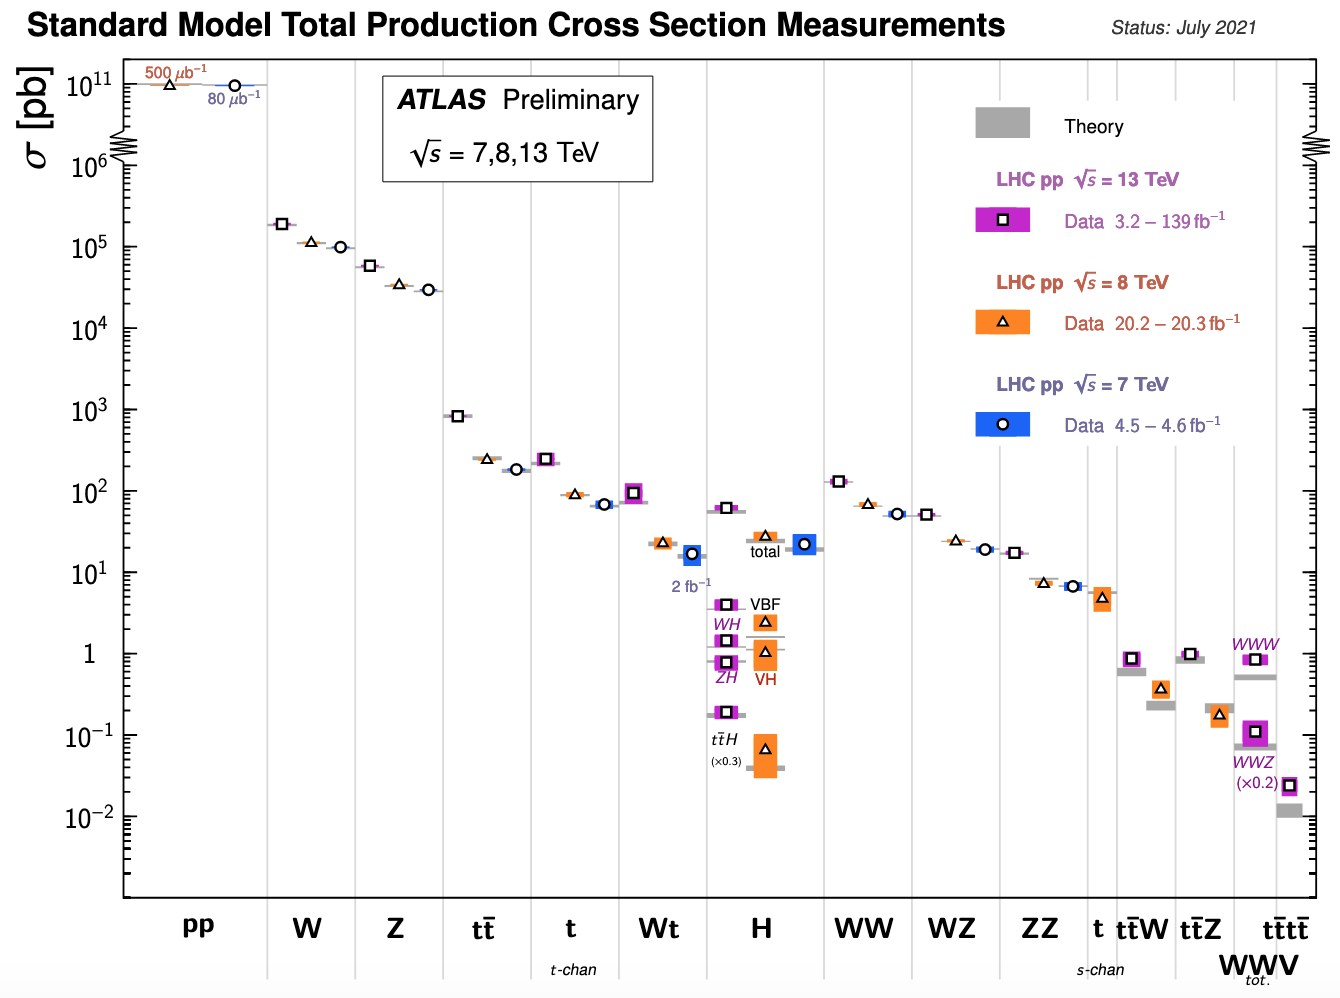
\includegraphics[width=0.8\textwidth]{Figures/3/ATLAS_xsections.png}
	\caption[]{Summary of Standard Model cross sections for particle production processes measured by the ATLAS detector. Figure from $\copyright$ \cite{ATL-PHYS-PUB-2021-032}.}
	\label{fig:ATLAS_xsections}
\end{figure}

\subsection{Branching Fractions and $W$ Boson Decays}

Unstable particles produced by the parton collisions will subsequently decay to less-massive particles, typically with multiple possible mechanisms, also known as ``channels", by which the decay can occur. Each such channel has an associated ``branching fraction", which quantifies the relative probability with which the decay will proceed by the given channel. The search presented in this thesis focuses on DM production in association with a pair of oppositely-charged W bosons. Figure \ref{fig:W_decays} shows the two $W$ boson decay routes. Due to energy and momentum conservation, W bosons can only decay to a pair of particles whose combined mass is smaller than the W mass. Charge conservation additionally requires that the decay products have a combined charge equal to that of the parent W boson. These two requirements allow the W to decay either to a quark-antiquark pair with one up-type quark/antiquark and one down-type, or to a charged lepton (L) and a neutrino ($\nu$).

\begin{figure}[H]
	\centering
	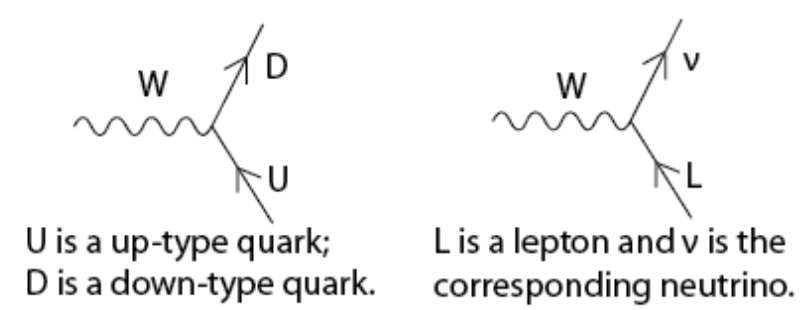
\includegraphics[width=0.5\textwidth]{Figures/3/W_decays.png}
	\caption[]{W boson decay mechanisms. Adapted from illustration by Garyzx, distributed under a CC BY-SA 3.0 license.}
	\label{fig:W_decays}
\end{figure}

\section{Experiments at the LHC}

The DM search presented in this thesis uses data collected from the ATLAS (A Toroidal LHC ApparatuS) detector \cite{atlas}. ATLAS is one of four particle detectors at the LHC which are designed to measure the energetic debris of particles produced by high energy particle collisions to perform precision measurements of the SM and search for new physics using the resulting particle collision data. This section briefly introduces each of the four particle detectors at the LHC, and what each contributes to the LHC physics programme.

The two largest, \textbf{ATLAS} (A Toroidal LHC ApparatuS) \cite{atlas} and \textbf{CMS} (Compact Muon Solenoid) \cite{cms}, are both general-purpose detectors designed to record all SM decay products from the collisions, with the exception of neutrinos which pass through due to their very low interaction cross sections. Thanks to their near-complete detection of decay products, data from these detectors can be used to study a wide range of physics processes resulting from the collisions, including both measurements of the SM and searches for new physics beyond the SM. While the physics goals of these two detectors are very similar, they are accomplished using different detector designs and technologies, and as such they are able to produce complementary physics studies.

The Large Hadron Collider beauty (LHCb) detector \cite{LHCb} is designed to measure heavy quark ($b$ and $c$) decays resulting from proton-proton collisions. Precise measurement of heavy quark decays are of particular interest for the study of CP violation in the SM, and in the search for potential sources of CP violation beyond the SM. Rather than providing full coverage of all collision products, the LHCb detector is comprised of a series of sub-detectors which provide ``forward angle" coverage to detect particles produced with a large boost along the direction of one of the two proton beams. This forward region is of particular interest for measurements of heavy quark decays, because this is the angular region in which heavy quark pairs are predominantly produced at high collision energy collisions.

A Large Ion Collider Experiment (ALICE) is designed to measure the products of heavy-ion collisions produced during special LHC runs in which the proton beams are replaced by Pb beams, which are collided a a centre of mass energy of 5 TeV. The high-energy Pb collisions produce a sufficiently high temperature and density to form an unbound state of quarks and gluons known as ``quark-gluon plasma". The study of this exotic sta



\section{Introduction to the ATLAS detector}

The ATLAS detector, shown schematically in figure \ref{fig:detector}, provides full 4$\pi$ coverage around the interaction point, with the exception of the beam pipe. It consists of several layers of sub-detectors, each of which is specialized for recording certain kinematic information and particle types. The sub-detectors are described in some detail below. 

\begin{itemize}
\item Introduction to the ATLAS detector, giving an idea of its scale and significance as one of the two general purpose particle detectors at the LHC (enables a wide range of physics measurement and search programmes; complementarity with CMS).
\item Inner detector $\rightarrow$ discussion of charged particle tracking will be relevant for later description of TAR jet reconstruction (may want to point that out already).
\item Calorimeters $\rightarrow$ emphasize distinction between small- and large-radius jets, and between electromagnetic and hadronic showers. 
\begin{itemize}
\item Talk about electron detection after/during the description of the EM calorimeter (should have all needed info since the inner tracker has already been discussed). 
\end{itemize}
\item Muon spectrometer for muon detection $\rightarrow$ emphasize that muons pass through the other sub-detectors. 
\item \met 
\begin{itemize}
\item Define \met here, now that all sub-detectors have been described. This intro to \met will be needed for the discussion of the \met trigger in the next section.
\item Shouldn't need to go into too much detail on the objects involved in \met reconstruction, since this will be covered in more detail in Chapter 5.
\end{itemize}
\item Trigger system 
\begin{itemize}
\item Discuss the relatively enormous cross sections of soft QCD processes $\rightarrow$ emphasize that much of the trigger design and data selections are devoted to reducing this soft QCD background to focus on the rarer physics processes of interest for measurements/searches. 
\item Otherwise, focus on the \met trigger, and mention that it only uses info from the calorimeter (relevant for later presentation of our use of the \met OR single muon trigger).
\end{itemize}
\end{itemize}
